\section{Battery Rack}
The battery rack in the robot located right above the motors in the frame. The number of batteries required for the operation of the robot is six batteries and the frame gave just enough room for the structure of the battery rack and the batteries themselves. The reason for the size batteries is because two are required to be connected in series to supply the controller with enough voltage to be split and supplying each motor with 25 volts. The proposal design of the battery rack to consist of 2"x2"x1/8" aluminum tubing but since Penguin ASI requested to use their spare material the tubing that was used was 2"x2"x1/4" aluminum tubing. The batteries are located at a height is near the top of the chassis which allowed the installer to have an easier job of placing the batteries in the frame from the original design. Since in the original design the installer had to place the batteries at the base of the frame which would put the installer at risk of injury. 
\subsection{Design Constraints and Functional Requirements}
The size of battery rack was constrained to the chassis that was provided. the available room that for the batteries in the frame was 1.82 m by 0.73 m. With this area six batteries were able to be placed in the frame in an orientation that had them all in line. Figure~\ref{fig:battery_rack_section} shows one section of the rack that holes two of the batteries. Since the batteries are places over the motors they had to be removable in order to access the components below. Having the racks removable was a functional requirement that needed to be met to allow the oil to be changed in the reductions when required and if motors were needed to be replaced.
\begin{figure}[htbp]
	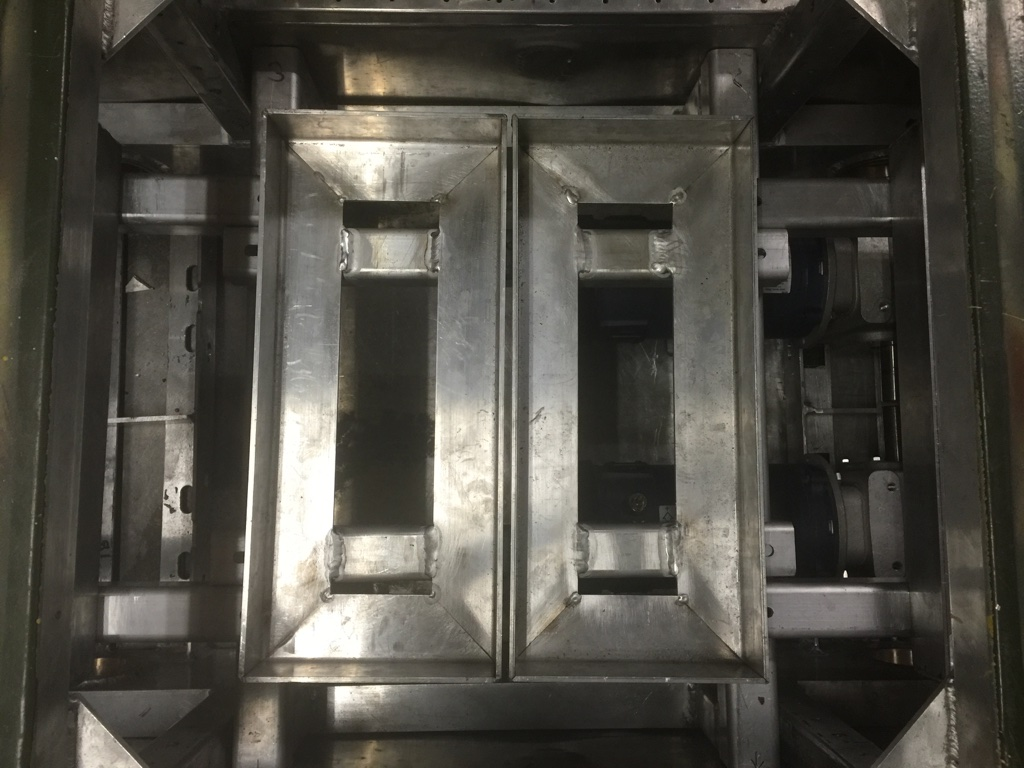
\includegraphics[width=\linewidth]{images/battery_rack_mid_bld.jpg}
	\caption{One section of three of the battery rack.}
	\label{fig:battery_rack_section}
\end{figure}
\subsection{Analysis and Design}
The changes made to the design from the proposal were that instead of using 1.5x1.5x1/8" tubing wall thickness for the members, 2x2x1/4" was used since this material was readily available at the Penguin ASI facility. This was an acceptable change since the increase in material thickness would only increase the strength of the structure and decreased the deflection when both 132.6 kg batteries were placed on the rack. The design was made into two components, the base component was welded to the frame and contains cross members that reach across from one side of the frame to the next in the 0.73 m span. The top section which contained the batteries used a thicker material then proposed just like the tubing for the base. The material used was 2x2x1/4" aluminum L beam instead of the 1/8" thickness stated in the proposal. This again only increase the strength of structure which made it an acceptable substitute. As can be seen in Figure~\ref{fig:battery_rack_section} the placement of the beams below the battery rack were orientated to allow the pairs of batteries to sit below the frame cut out at the top. The slots that can be seen allow this alignment to be possible, so they can be adjusted.
\subsubsection{Battery Mounts}
\subsubsection{Battery Support Frame}
